% !TEX program = xelatex
% !TEX options = --shell-escape -synctex=1 -interaction=nonstopmode -file-line-error "%DOC%"
\documentclass[12pt]{article}
\usepackage[UTF8]{ctex}
\usepackage{biblatex}
\usepackage{amssymb}
\usepackage{latexsym}
\usepackage{amsmath}
\usepackage{cases}
\usepackage{geometry}
\usepackage{graphicx}
\usepackage{float}
\usepackage{listings}
\usepackage{enumerate}
\usepackage{color}
\usepackage{xcolor}
\usepackage{plantuml}
\usepackage{hyperref}
\usepackage{pifont}
\usepackage{tabularx,ragged2e}

\renewcommand\tabularxcolumn[1]{m{#1}}% 表格简直居中
\newcolumntype{C}{>{\Centering\arraybackslash}X} % 定义单元格水平居中
\renewcommand{\contentsname}{\centerline{ 目\quad 录}}

\hypersetup{
    pdfauthor={张三丰},
    pdftitle={大明武当山文化有限公司},
    pdfencoding=auto,
    bookmarksopen=true
}
\colorlet{keyword}{blue!100!black!80}
\colorlet{comment}{green!90!black!90}
%先自定义三种颜色
\definecolor{dkgreen}{rgb}{0,0.6,0}
\definecolor{mauve}{rgb}{0.58,0,0.82}
\lstset{frame=tb,
  language=Java,
  aboveskip=3mm,
  belowskip=3mm,
  showstringspaces=false,
  columns=flexible,
  basicstyle={\small\ttfamily},
  numbers=none,
  numberstyle=\tiny\color{gray},
  keywordstyle=\color{blue},
  commentstyle=\color{dkgreen},
  stringstyle=\color{mauve},
  breaklines=true,
  breakatwhitespace=true,
  tabsize=3,
  numbers=left,
  frame=single
}
\addbibresource{bib.bib}
\setlength{\parindent}{2em}
\bibliography{bib}
\geometry{a4paper,scale=0.8}
\linespread{1.5}
\graphicspath{{assets/}}

\begin{document}

\begin{titlepage}
\begin{center}
\linespread{1.2}\huge {\bfseries 大明武当 \\ \ding{72} \ding{72} \ding{72} \ding{72} \ding{73}}\\[1cm]
\linespread{1}
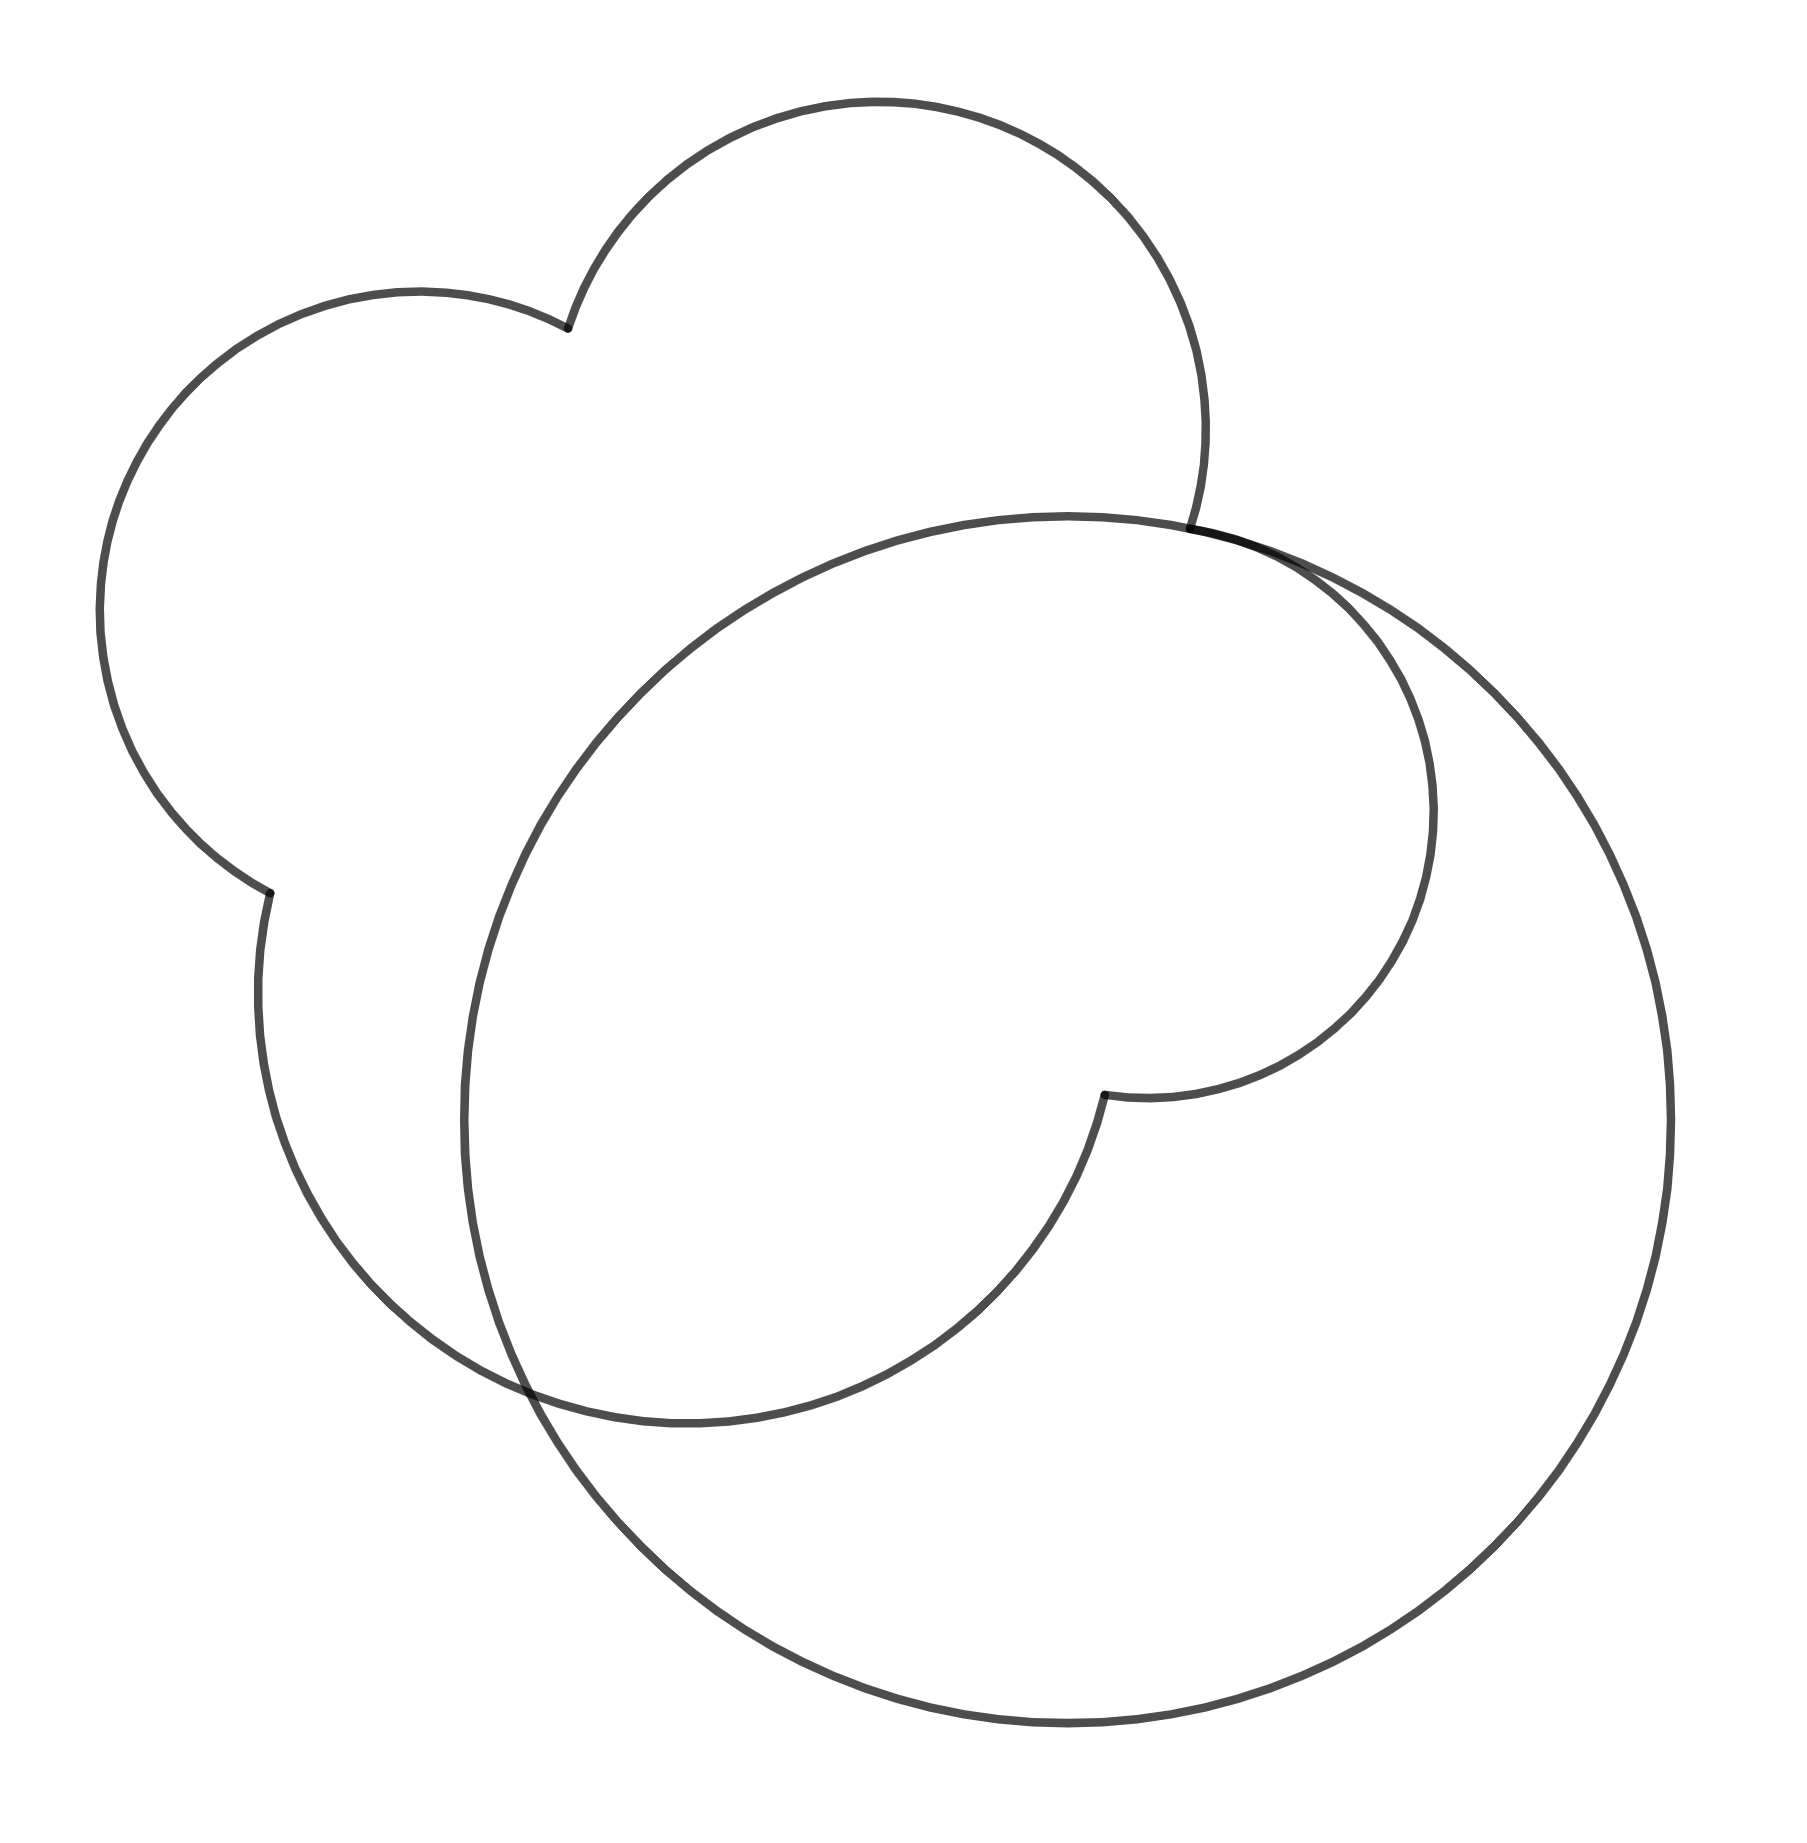
\includegraphics[height=2.9cm]{logo.png}\\[2cm]
\linespread{1.9}\huge {\bfseries 当前大明武林形势分析}\\
\linespread{1.9}\LARGE {\bfseries 武当的抉择}\\[2.5cm]

{\Large 主持小组}\\[0.3cm]
\Large 张三丰\\[4cm] 
\large 2022年3月3日
\end{center}
\end{titlepage}

\tableofcontents

\section{整体说明}

\begin{figure}[H]
  \centering
  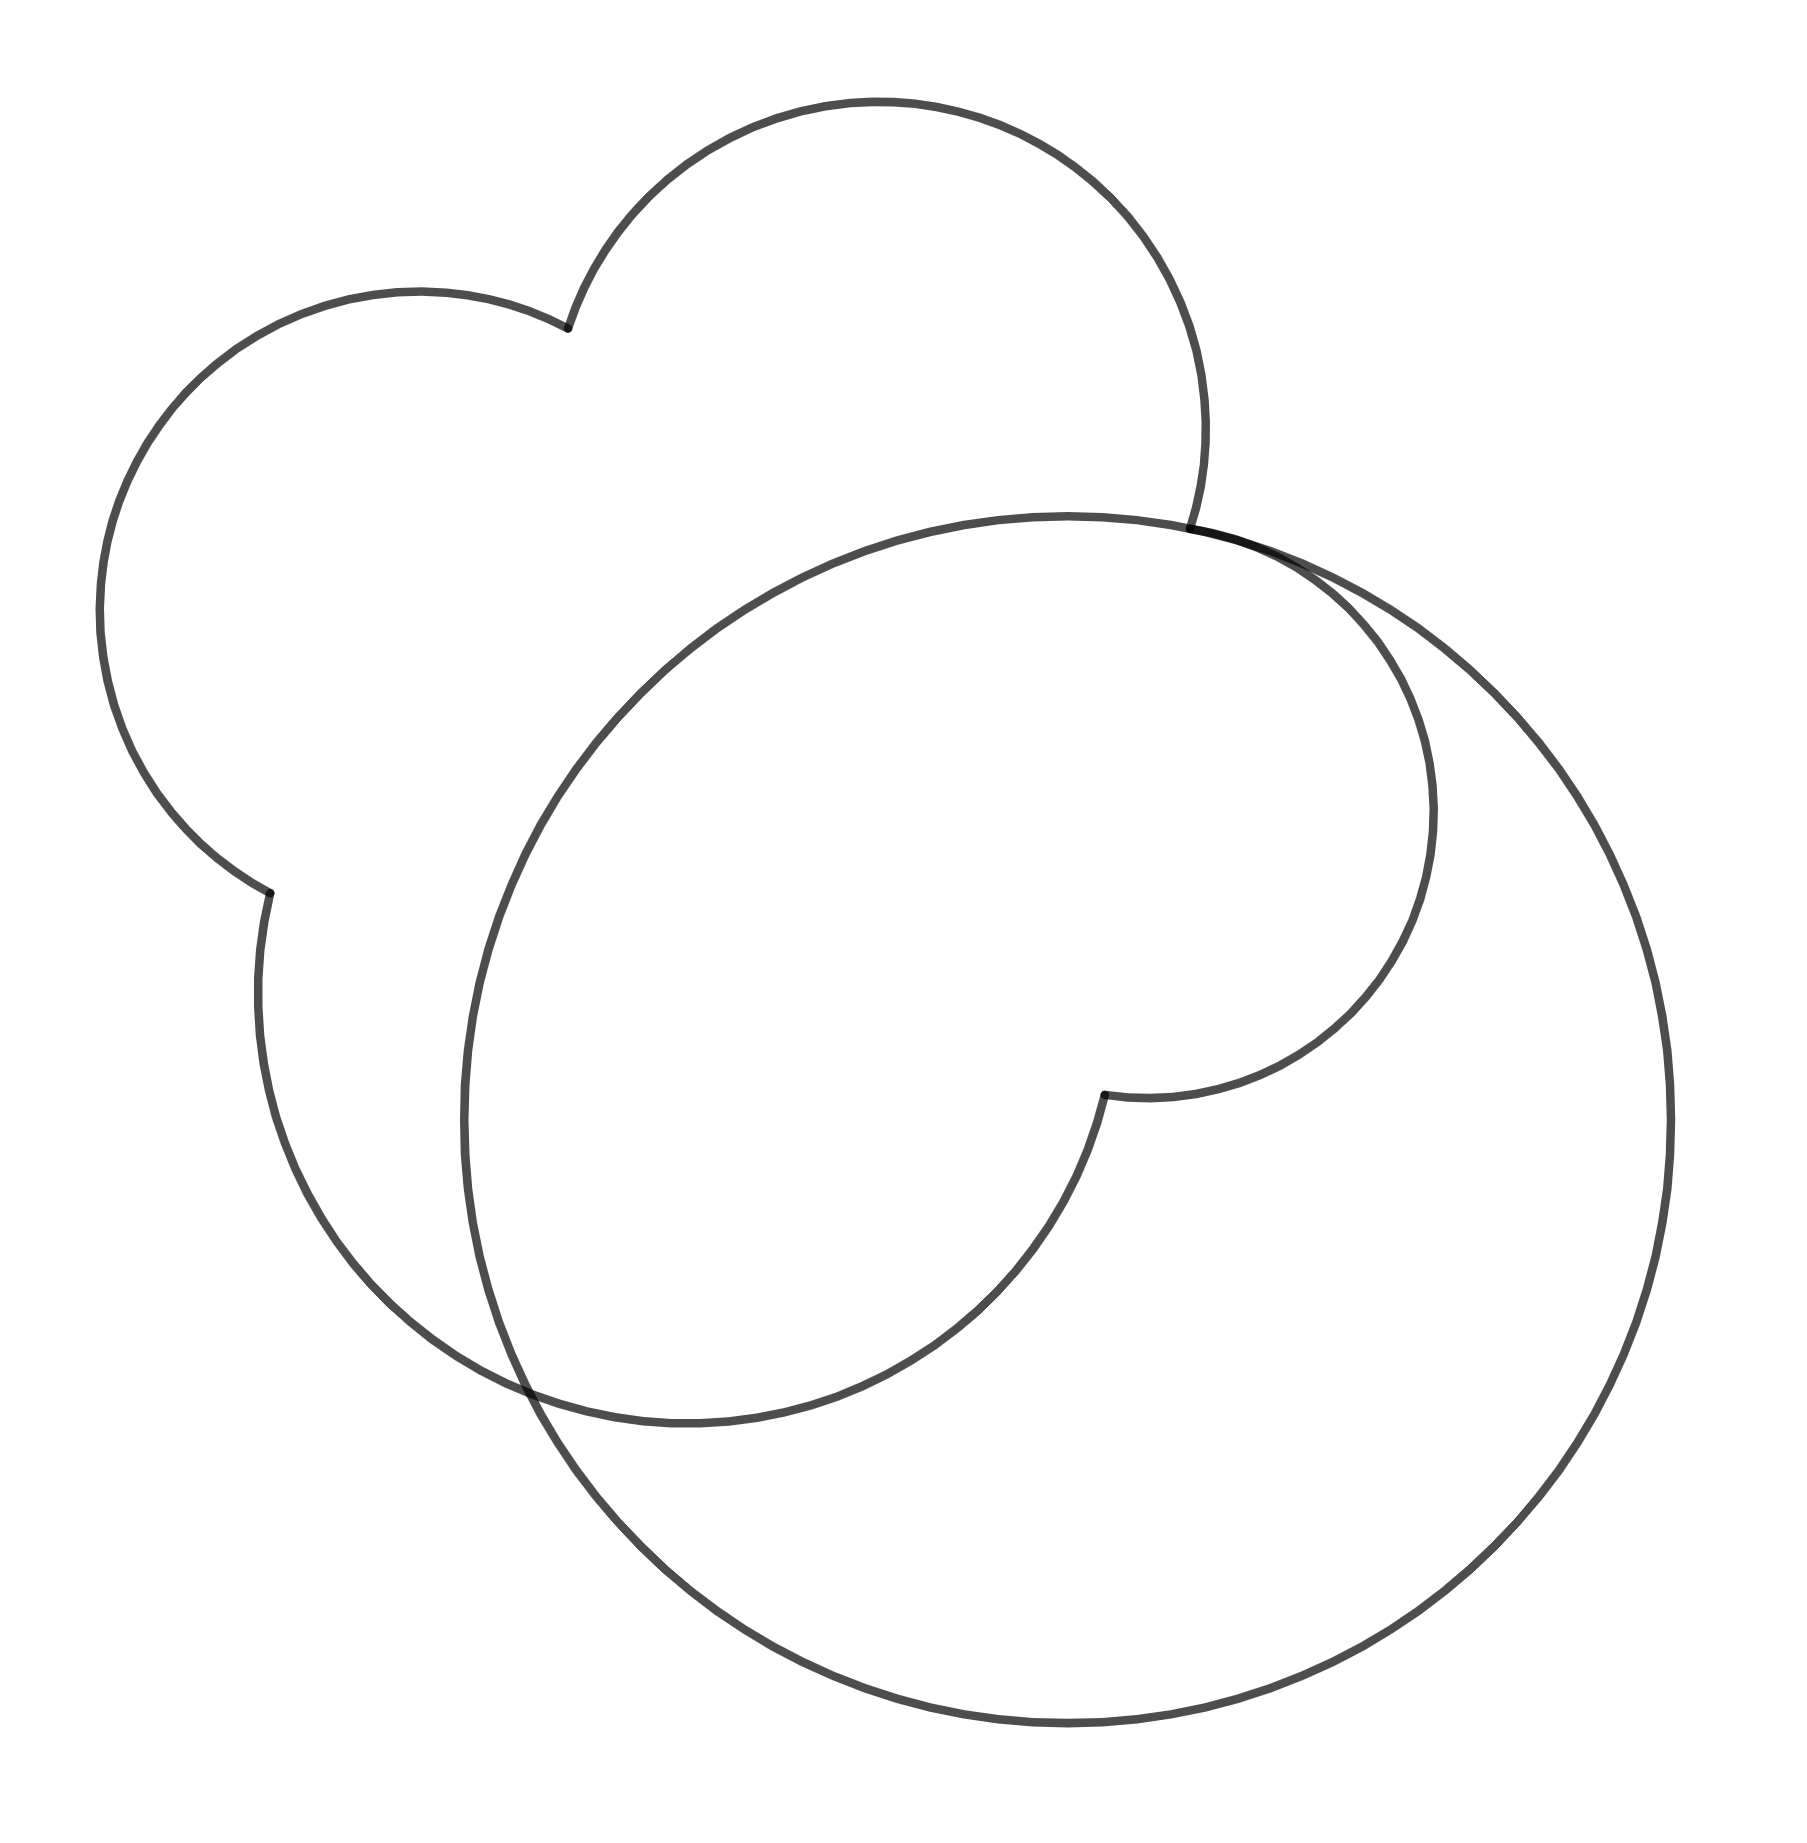
\includegraphics[width=\textwidth]{logo.png}
  \caption{整体图片}
  \label{整体图片}
\end{figure}

\begin{table}[H]
  \centering  % 显示位置为中间
  \caption{整体说明表}  % 表格标题
	\label{整体说明表}  % 用于索引表格的标签
  \begin{tabularx}{\textwidth}{|c|c|X|}
    \hline
    门派名称 & 编码 & 说明\\
    \hline
    大明武当山 & 09 & 注册后发展较好\\
    \hline
    少林文化传娱有限公司 & 08 & 注册后发展奇好,当前极为兴旺,方丈有钱\\
    \hline
    黑木崖安保集团 & 10 & 未注册企业\\
    \hline
  \end{tabularx}
\end{table}

如图\ref{整体图片}、如表\ref{整体说明表}

\section{正文}

\end{document}
